% Chapter Template

% Main chapter title
%\chapter[toc version]{doc version}
\chapter{System Architecture \& Design}

% Short version of the title for the header
%\chaptermark{version for header}

% Chapter Label
% For referencing this chapter elsewhere, use \ref{ChapterTemplate}
\label{Chapter4SystemArchitectureDesign}

% Write text in here
% Use \subsection and \subsubsection to organize text

This chapter outlines the architecture of the proposed system, detailing the key components and how they interact to enable 
evaluation of student-submitted network exercises.

The system is designed to provide each student with a working environment where custom virtual network topologies can be 
deployed, configured, and tested. To achieve this, the platform integrates several technologies—such as\ac{gns3} for network 
emulation,\ac{pve} for virtualization, and Nornir for configuration testing—alongside an asynchronous web-based\ac{api} layer for 
user interaction and system communications.

This section provides a high-level overview of the system, the rationale behind its design choices, and the fundamental 
components that make up its architecture.

\section{Functional Use Cases}

\section{System Architecture Overview}
    The architecture is divided into several key components, each responsible for a specific aspect of the system's functionality. 
    The main components of the system architecture are as follows:

    \begin{itemize}
        \item \textbf{Web Application:} The web application serves as the main interface for users to interact with the system. It provides 
        endpoints for, amongst others, evaluation, creation  and viewing available exercises. The application is designed to be asynchronous 
        where possible, allowing for efficient handling of multiple requests simultaneously.
        
        \item \textbf{Proxmox VE:}\ac{pve} is responsible for creating and managing\ac{vm}s that host the network devices used in 
        the exercises. This component interacts with the web application and all communication is done asynchronously through 
        the\ac{pve}\ac{rest}\ac{api}, which allows for efficient communication, keeping the web application responsive, while also 
        keeping the components decoupled.
        
        \item \textbf{GNS3:}\ac{gns3} is used to emulate all the components of the virtual networks to be configured by students, 
        using various types of virtualization detailed earlier. Communication with\ac{gns3} is done through 
        the\ac{gns3}\ac{rest}\ac{api} by the web application during template\ac{vm} creation and validation

        \item \textbf{Nornir:} This automation framework is used for validating device configurations. It connects to the 
        virtualized devices, executes commands, and compares the output to expected results to determine correctness.
        Currently this component is integrated into the web application
    \end{itemize}

\section{Proxmox VE}

    \ac{pve} functions as the virtualization backbone of the system, enabling the creation and management of Linux-based\ac{vm}s 
    which in turn host services for use by students. Each\ac{vm} runs a lightweight Linux-based operating system with a 
    dedicated\ac{gns3} instance, providing a self-contained environment for deploying and configuring virtual networks 
    and their components.

    All\ac{pve}-related operations—such as cloning, starting, templating, and deletion—are fully automated and triggered by the 
    web application. Under normal operation ,after doing pre-required setup, no further manual intervention using the\ac{pve} web 
    UI or shell utilities is required; such intervention is only necessary when the system's error handling mechanisms detect failures 
    that cannot be automatically resolved. To securely execute these operations, the application authenticates to the\ac{pve}\ac{api} 
    using token-based authentication. The required credentials and configuration parameters are securely injected via environment variables\unsure{this may change}, 
    while the time limited token is stored in memory, ensuring that only authorized and properly configured processes can interact 
    with the\ac{pve} infrastructure.

    \subsection{Why Proxmox VE?}

        \ac{pve} was chosen for several compelling reasons that make it ideal for it to be choosen as our virtualization platform. First, 
        it's completely free to use for all core functionality, with no hidden costs or licensing traps. Unlike proprietary solutions that 
        charge per CPU core or socket,\ac{pve} lets us scale up our infrastructure without worrying about surprise licensing fees.

        The platform's support for both containers and\ac{vm}s within a single management interface gives us tremendous flexibility. We 
        can run lightweight\ac{lxc} for applications that dont require a full\ac{vm} while using full\ac{vm}s where required seamlessly. 
        This hybrid approach would not be as straightforward with other solutions, like VMware ESXi.

        We also value storage system's flexibility with LVM-thin provisioning allows efficient snapshotting of student environments while 
        maintaining good performance.

        Looking ahead,\ac{pve}'s built-in support for emerging technologies like software-defined networking and its robust role-based 
        access control system means our project still has room to grow into\ac{pve}. The active open-source development community ensures 
        continuous improvements without vendor lock-in.

    \subsection{Proxmox VE Limitations}

        During development, we encountered several challenges when interfacing programmatically with\ac{pve}. One of th most significant 
        issues stemmed from the platform's limited visibility into non-instantaneous operations - particularly for tasks like\ac{vm} cloning, 
        where the system did not provide task ids in the\ac{http} responses. This forced us to implement custom polling mechanisms to reliably 
        determine operation completion states where possible.

        A more critical limitation emerged in\ac{pve}ac{rest}ac{api}'s resilience characteristics. During stress testing, we discovered that 
        even moderate request volumes done using a single machine running sequential code could overwhelm the single-node cluster's management 
        daemon, triggering frequent\ac{http} 500 errors. These reliability constraints necessitated the development of protective measures 
        including exponential backoff retry logic and strict client-side concurrent request limiting to maintain system stability.

    \subsection{Proxmox VE Firewall}

        \ac{pve} comes bundled with a iptables-based firewall implementation that can be enabled and configured at different levels.

        The Proxmox host-level firewall provides essential features for securing student work environments, during examination 
        periods, preventing student machines and the virtualized network equipments in them from communicating with outside networks.

        This is done by adding firewall rules at the host level, meaning to each relevant student\ac{vm}, that disable communications
        in both directions, with the exception of the machine that is responsible for configuration validation.

        By default this behavior is not active and must be enabled on an as-needed basis, typically when a controlled assessment 
        environment is required for more rigorous situations such as examinations.

        In future iterations it may also be valuable to develop this further and making this feature less rigid as it may be interesting 
        to have exercises that communicate with devices on the internet.
    
    \subsection{Exploration of containers as a full substitute for VMs}

        During development, we attempted to minimize\ac{vm} usage where possible to accommodate as much scaling potencial as possible. 
        The introduction of the\ac{gns3} web interface allowed the machines hosting\ac{gns3} instances to operate in a headless manner, 
        removing the need for direct student interaction with the host machine. This eliminated desktop environment requirements and 
        significantly reduced memory overhead, improving scalability.

        We further explored replacing\ac{vm}s entirely with containers, which promised additional resource savings. However, this approach 
        proved unworkable due to fundamental technical constraints. Effective emulation requires\ac{kvm} acceleration, which presents 
        two problematic scenarios in containerized environments: either running unprivileged containers without\ac{kvm} access (resulting 
        in unacceptable performance degradation) or configuring privileged containers or containers with\ac{kvm} passthrough (introducing 
        serious security vulnerabilities).

        Given that software emulation without\ac{kvm} acceleration delivers poor performance for interactive use, we abandoned containerization 
        as a complete\ac{vm} replacement. The\ac{vm}-based architecture remains necessary to maintain both performance through hardware 
        acceleration and proper isolation between student environments.

        \subsubsection{VM Lifecycle}

            The lifecycle of a\ac{vm} begins when a new exercise is created by a priviledged user through the web application. 
            Upon exercise creation, the platform automatically clones a pre-configured base template\ac{vm} stored in\ac{pve}. This new instance 
            undergoes a configuration process where the provided\ac{gns3} project file is imported and a series of user-defined commands are executed 
            across the provided network topology. Once the setup is finalized, the configured\ac{vm} is converted into a new template\ac{vm} that 
            is tailored to that exercise.

            When students are enrolled in an exercise, the system generates individual work environments, by creating linked clones from these 
            exercise-specific templates. Each student receives their own isolated\ac{vm} instance that precisely mirrors the original template's 
            configuration. This cloning approach ensures both consistency across student environments and rapid provisioning, as linked clones 
            avoid the overhead of full disk copies while maintaining the template's baseline configuration. The use of linked clones significantly 
            reduces both storage requirements and deployment time compared to traditional full cloning methods.
        
\section{GNS3}

    \ac{gns3} serves as the core network virtualization component in our system, providing the capability to emulate various network devices 
    and topologies. The platform was selected for several key advantages: its remote web-based interaction, the intuitive drag-and-drop interface 
    simplifies usage, and its broad device support accommodates both terminal-based and GUI network equipment and full computers. Additionally, 
    \ac{gns3}'s\ac{api} allows for programmatic interaction, which proves essential for automation within our environment.

    Currently, the system requires manual preparation of the base \ac{gns3} template\ac{vm}. During initial setup, an administrator must first create 
    and configure a new\ac{vm}, then proceed to install and set up the\ac{gns3} environment. The final preparation step involves importing all 
    necessary device images, including routers, switches, and other equipment that will be available for student exercises.

    This base template then serves as the source for all subsequent student instances through\ac{pve}'s cloning functionality. While this 
    manual setup process adds initial configuration overhead, it ensures complete control over the base environment and allows for careful 
    curation of the included device images.

    The system achieves scalability through multiple \ac{vm} instances running in \ac{pve}, each hosting an independent \ac{gns3} environment. 
    This architecture enables concurrent usage by multiple students on a single physical host. For future expansion, the design supports 
    horizontal scaling by adding additional nodes to the \ac{pve} cluster, allowing the platform to accommodate growing numbers of users 
    without requiring complete architectural changes.

    \begin{figure}
        \centering
          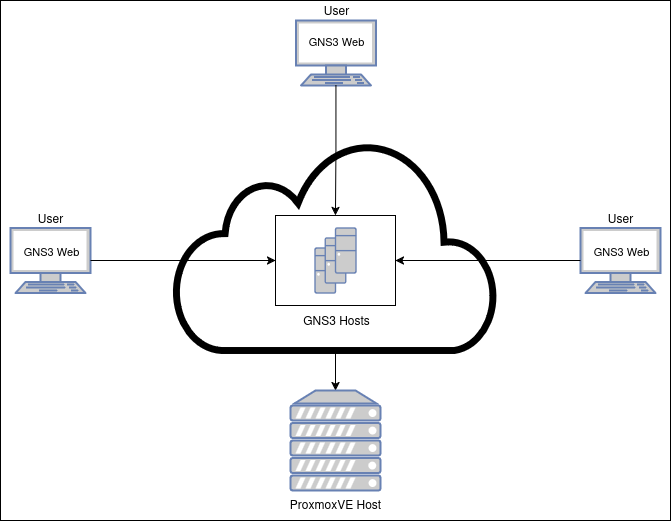
\includegraphics[width=.95\linewidth]
            {4SystemArchitectureDesign/user-gns3-proxmox-diagram.png}
        \caption{A diagram showcasing how users interact with the system's resources on a high level}
      \hfill
    \end{figure}

\section{High-level architecture}

    \subsection{Available Hardware}

        The current deployment hosts all internal system components (those shown in the architecture diagram excluding the external LDAP instance) 
        on a single physical server with the following specifications.

        \begin{table}[h]
            \centering
            \caption{System Hardware Specifications}
            \begin{tabular}{|l|l|}
                \hline
                \textbf{Component} & \textbf{Specification} \\ \hline
                Processor & Intel Core i7-9700K \\ \hline
                Memory & 32GB DDR4 @ 2666MHz \\ \hline
                Storage & 1TB Samsung 970 EVO Plus NVMe SSD \\ \hline
                Graphics & NVIDIA GTX 1650 \\ \hline
            \end{tabular}
        \end{table}

        This machine's specifications, while capable enough for development purposes, create inherent memory constraints. With 32GB of available RAM, 
        practical\ac{vm} allocation becomes the primary bottleneck. For instance, when deploying\ac{gns3} instances each configured with 4GB of memory, 
        the system can maintain only seven active\ac{vm}s simultaneously. This limitation accounts for the\ac{pve} hypervisor's own memory overhead 
        before inducing SWAP file usage, which would degrade performance.

    \subsection{User Interface}
        The system employs a dual-interface web architecture accessible through standard browsers. For administrative functions and exercise management, 
        users interact with Jinja2-rendered HTML pages delivered by the web application. These templates handle all developed features, like user 
        authentication,\ac{vm} interaction etc.

        When working on networking exercises, users can transition to the \ac{gns3}-web interface by clicking a button. This dedicated environment 
        provides direct access to the user's virtual network devices, as required by each exercise scenario. This integration ensures users experience 
        a cohesive workflow from exercise selection to practical implementation without needing multiple authentication steps or application switches.

    \subsection{Web Application}

        The web application serves as the primary interface through which users interact with the system. It is built using the FastAPI 
        framework, following a migration from an earlier prototype developed using Flask, and follows an asynchronous-first, modular 
        architecture that provides scalable interactions with other system components.

        The application exposes a\ac{rest}\ac{api} that supports endpoints for user authentication, exercise creation, virtual 
        machine management, and configuration validation. It acts as the coordinator for the entire system, triggering operations 
        in\ac{pve},\ac{gns3}, and Nornir based on user actions.

        Wherever possible, asynchronous I/O is employed to prevent blocking during operations such as\ac{api} calls to\ac{pve}.
        Multiprocessing is also utilized to handle configuration validation. This keeps the system responsive and performant, 
        especially when handling multiple simultaneous requests from different users.

        Internally, the application is designed to be stateless and maintain minimal runtime state.  Most essential information—such 
        as user accounts, defined exercises, and student-to-VM mappings—is persisted in a relational database rather than stored in 
        memory. Configuration values such as API tokens, base URLs, and database credentials are injected via environment variables 
        to decouple deployment-specific settings from the application code. This design improves reliability, supports concurrent 
        usage, and enables horizontal scalability if deployed across multiple instances. 

        To ensure maintainability and modularity, interactions with external services like\ac{pve} and\ac{gns3} are isolated in 
        dedicated modules. These serve as abstraction layers between the application logic and third-party\ac{api}s, exposing clean, 
        reusable interfaces while hiding low-level implementation details. For example,\ac{pve}-related operations such as\ac{vm} 
        creation and deletion are handled in a separate module (e.g services/proxmox.py), as are all\ac{gns3}-related tasks. This 
        separation of concerns improves the structure of the codebase and simplifies future maintainability by being more readable.

        To help with development and testing, the application automatically generates OpenAPI-compliant documentation, allowing 
        developers to explore and interact with available endpoints. This self-documenting behavior streamlines integration 
        testing and encourages a more agile development process.

        Finally, to safeguard user data and infrastructure control points, the application enforces secure authentication mechanisms 
        using\ac{jwt} ensuring that only authorized users can trigger actions on shared resources.

    \begin{figure}
        \centering
            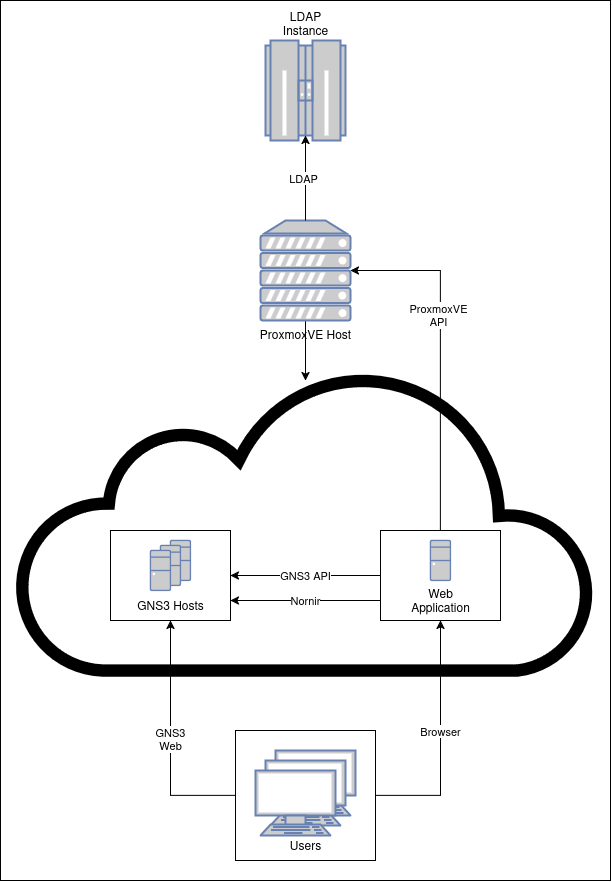
\includegraphics[width=.95\linewidth]
                {4SystemArchitectureDesign/system-diagram.png}
            \caption{A diagram showcasing a high level overview of the system's main components}
        \hfill
    \end{figure}

    \subsection{Virtualization Components}

        The system employs a hybrid virtualization approach using\ac{pve} as the foundational platform. The usage of containers was 
        explored but it was found unsuitable for our main use case of virtualization,\ac{gns3} instances. However there remains one valid 
        usage for containers for the project, which is hosting the web application. However this component may also be optionally hosted in 
        a separate physical machine.

        For network emulation, the system utilizes full\ac{kvm}-based virtual machines, each hosting a\ac{gns3} instance. These\ac{vm}s 
        provide the necessary hardware virtualization support for nested device emulation, particularly crucial for fast virtualization. 
        Finally, by the use of linked clones and storage-efficient backing filesystems, in this case LVM-thin, allows the system to rapidly 
        provision\ac{vm}s while minimizing storage usage.
    
    \subsection{Evluation component}

        The system employs a modular evaluation framework built on Nornir to validate configurations across virtualized network devices. 
        At its core, this component utilizes specialized Python classes called "modules" that encapsulate platform-specific validation logic. 
        Each module is responsible for three key functions: identifying the target device's platform (such as Cisco IOS, Linux, or VPCS), 
        executing the appropriate validation commands for that platform, and interpreting the command output using regular expressions to d
        etermine configuration correctness.

        The architecture follows an object-oriented design pattern with a base \texttt{CommandModule} class that handles common functionality. 
        This parent class manages the Nornir inventory initialization and provides essential methods like platform detection and command execution. 
        The actual validation logic is implemented in child classes that inherit from \texttt{CommandModule}, with each subclass specializing in 
        a particular type of network test. For example, the included \texttt{PingModule} implements platform-specific variants of the ping command 
        and corresponding response interpretation methods. This design promotes code reuse while allowing easy extension for new test types, as 
        developers can create additional modules by simply extending the base class and implementing the required platform-specific methods.
        
        Configuration validation occurs through a multi-stage process. When a test is initiated, the system first identifies the target device's 
        platform through Nornir's inventory system. It then dispatches the appropriate platform-specific command variant, such as the Cisco IOS-style 
        ping command for routers versus the Linux \texttt{ping -c} syntax for Linux hosts. The module captures and sanitizes the raw command output, 
        removing terminal control sequences and other artifacts before applying regular expressions to assess the results. For connectivity tests like 
        ping, the interpretation logic calculates success rates against a configurable tolerance threshold defined in the system constants.
        
        The evaluation framework supports several advanced features to enhance reliability and debugging. Command timeouts are managed to prevent 
        hanging operations, with a default window that can be tuned as needed. Future extensions could incorporate snapshot functionality, allowing 
        the system to capture and compare device states at different points during an exercise, though this capability is not currently implemented 
        in the base version. The modular architecture ensures such enhancements can be added without disrupting existing validation workflows.

    \subsection{Storage component}
        
        The system has two main components regarding storage, one for the database needs of the web application and one for the disks of the \ac{vm}s.

        \subsubsection{Virtual machine storage}

            \ac{lvmt} is an efficient solution for creating and managing virtual machines (VMs) by optimizing storage usage and improving performance. Unlike 
            traditional\ac{lvm}, which pre-allocates disk space,\ac{lvmt} allows dynamic allocation, meaning storage is consumed only as the\ac{vm} writes 
            data—ideal for environments like ours where multiple \ac{vm}s share the same storage pool. When combined with\ac{cow} snapshots, \ac{lvmt} enables 
            rapid\ac{vm} cloning and backup operations. For instance, a base\ac{vm} image can serve as a template, and new\ac{vm}s are created as linked 
            clones that initially share all data blocks with the original. Only when a\ac{vm} modifies its disk does\ac{lvmt} allocate new blocks, 
            significantly reducing storage overhead. This approach not only saves disk space but also speeds up\ac{vm} deployment, making it a great choice for 
            our project. Additionally, since snapshots are space-efficient, in the future, we can maintain multiple VM checkpoints without worrying about excessive 
            storage consumption—as long as the thin pool is monitored to avoid overprovisioning. Overall,\ac{lvmt} provides a scalable, high-performance storage 
            layer for virtualization with minimal waste.

        \subsubsection{Web application database}

            The SQLite database serves as the central repository for all application data, leveraging SQLModel as an ORM layer that combines Pydantic 
            validation with SQLAlchemy's database capabilities. This hybrid approach provides both runtime type safety and efficient database operations, 
            while Alembic handles schema migrations to accommodate evolving data requirements.

            The database schema organizes information across several interrelated models. User management builds upon a base \texttt{CustomBase} class 
            that automatically tracks creation timestamps, with the \texttt{User} model storing authentication credentials, administrative privileges, 
            and relationships to both submissions and virtual machine instances. The \texttt{Exercise} model captures lab configuration details, including 
            \ac{json}-serialized validation rules and device configurations stored as text fields due to SQLite's native type limitations.\ac{vm} 
            provisioning is managed through the \texttt{TemplateVm} and \texttt{WorkVm} hierarchy, where template instances maintain the base\ac{gns3} 
            project configurations and spawned work environments link back to both users and exercises. The \texttt{Submission} model completes the 
            core data structure by tracking student attempts, scores, and evaluation outputs while maintaining referential integrity through SQLModel 
            relationships.

            \begin{figure}
                \centering
                    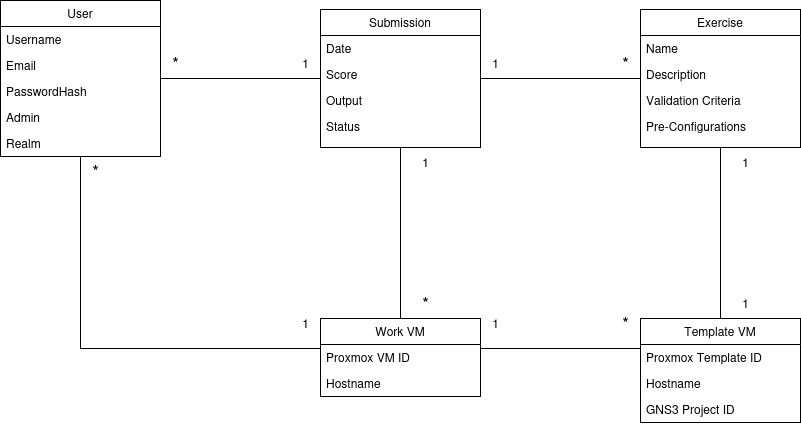
\includegraphics[width=.95\linewidth]
                        {4SystemArchitectureDesign/db_er.png}
                    \caption{A diagram of our database}
                \hfill
            \end{figure}


\section{FastAPI Adoption: Overcoming Flask's Shortcomings}

    \subsection{Initial setup: Flask}

        Initially, Flask served as the framework for the web application, providing the necessary infrastructure to handle \ac{http} 
        requests, render templates, and manage application routing. Its flexibility and minimalistic approach allow for the 
        integration of various extensions and libraries as needed, ensuring the application remains lightweight yet functional. 
        Flask's comprehensive documentation and supportive community further enhance its suitability by the creation and support
        of community-driven extensions speeding up development and reducing the need to reinvent the wheel.

        However, as development progressed, the need for better I/O performance became increasingly apparent. Early on, it was 
        clear that leveraging Python's native \textttt{asyncio} would benefit the project—but a significant portion of the existing codebase, 
        including Flask itself, relied on non-async-compatible libraries. This limitation stemmed from Flask's foundation on\ac{wsgi}, a 
        synchronous standard developed long before Python's asyncio was introduced.\ac{wsgi} operates strictly in a blocking request-response 
        model, requiring each request to complete fully before processing the next. While traditional workarounds like multi-threading 
        or multi-processing can mitigate this, they introduce complexity and are better suited for CPU-bound tasks than I/O-bound workloads.

        To address these constraints, several approaches were considered:

        \begin{itemize}
            \item \textbf{Gevent/Eventlet:} These libraries use monkey-patching to emulate asynchronous behavior in synchronous code. However, 
            they are not true asyncio and can lead to unpredictable behavior. Given the project's early stage, this option was deemed too risky

            \item \textbf{Flask + Celery:} Offloading long-running tasks to Celery workers helps avoid blocking but introduces operational overhead, 
            requiring additional infrastructure like Redis or RabbitMQ for message brokering

            \item \textbf{Quart (ASGI Flask):} A Flask-compatible\ac{asgi} reimplementation with native async/await support. However, Quart lacks 
            Flask's mature ecosystem and still relies partially on monkey-patching, raising concerns about long-term stability

            \item \textbf{FastAPI (Full ASGI migration):} Built on\ac{asgi}, FastAPI was designed with async-first principles, enabling efficient handling 
            of thousands of concurrent connections. Its native async/await support and modern tooling offer a cleaner solution without the need 
            for workarounds, at the expense of having to reimplement some features already implemented in Flask
        \end{itemize}

        While Flask remained suitable for early development, emerging requirements—particularly those involving asynchronous 
        communication for more scalable I/O operations—eventually led to a need to explore architectural shifts, due to 
        Flask's limited async support and\ac{wsgi} heritage. 
    
    \subsection{Second setup: Flask + Celery}

        As the limitations of Flask's synchronous\ac{wsgi} model became more apparent, we explored Celery as a potential solution for handling 
        asynchronous tasks. Celery, a distributed task queue system, allows offloading blocking I/O to separate worker processes. 
        Celery operates by decoupling task execution from the main application flow. When a time-consuming operation is required, Flask 
        dispatches it to a Celery worker via a message broker (typically Redis or RabbitMQ). The worker processes the task asynchronously, 
        while Flask remains free to handle incoming requests. While this approach mitigated some of Flask's blocking I/O issues, it 
        introduced new challenges in complexity and system overhead.

        The Celery architecture operates through worker processes that listen to the message broker for tasks. These workers run as 
        independent processes, executing tasks marked with Celery's \texttt{@app.task} decorator. The system's concurrent processing 
        capability comes from multiple workers operating in parallel, each handling different tasks from the queue. Tasks are Python 
        functions that are decorated with provided Celery decorators such as \texttt{@app.task}, causing them to be registered as 
        Celery tasks within the Celery application. This design is particularly valuable for operations like batch processing or 
        scheduled jobs that would otherwise block Flask's synchronous request handling.

        \begin{algorithm}
            \caption{Calling a Celery Task and Getting the Result}\label{celery-call-result}
            \begin{algorithmic}[1]
            \State \textbf{from} celery \textbf{import} Celery
            \State
            \State \textbf{app} = Celery('tasks', broker='redis://localhost:6379/0', backend='redis://localhost:6379/0')
            \State
            \State \textbf{@app.task}
            \State \textbf{def} hello():
            \State \hspace{1em} \textbf{return} 'hello world'
            \State
            \State \textbf{result} = hello.delay()
            \State \textbf{print}(result.get())
            \end{algorithmic}
        \end{algorithm}

        To execute a task, a Celery task function must be called using the \textit{delay()} method, which will return a result object. 
        This result object can be used to check the status of the task and to retrieve the result once it is available.

        Celery supports horizontal scaling by design, allowing multiple worker pools to run on separate physical or virtual machines. 
        This makes it especially effective for handling growing workloads—for example, processing email newsletters for an expanding 
        user base.

        Celery's advanced features, including task retries, chaining, and prioritization, while powerful, further increased the 
        system's complexity. We found ourselves managing not just our application logic, but also the reliability of the message broker, 
        persistence of results, and supervision of worker processes. This architectural overhead seemed increasingly disproportionate to 
        our actual needs as the project evolved.

        Furthermore, Celery clients and workers introduce a non-negligible overhead in terms of CPU and memory usage, even when 
        idle, as they must maintain persistent connections to the broker and periodically perform health checks or heartbeats. 
        This can be a concern in resource-constrained environments or during development.This overhead became especially evident 
        during early integration tests.

        As the project evolved and tests were performed, it became increasingly clear that Celery's benefits lend themselves better 
        to CPU-bound workloads, as opposed to our I/O-bound ones, and they did not outweigh its resource and architectural costs for 
        the current use case. This realization prompted an exploration of more lightweight asynchronous alternatives, eventually 
        culminating in an investigation into \ac{asgi}-compliant frameworks with native async capabilities and simpler concurrency 
        management.

    \subsection{Third setup: Quart, an ASGI-compliant Flask reimplementation}

        Quart emerged as a promising candidate during our exploration of async solutions, offering a unique combination of 
        Flask syntax with\ac{ASGI} compliance. As a near-drop-in replacement for Flask, Quart theoretically allowed for 
        an easy migration while providing all the benefits of native async/await support. The framework's design promised 
        seamless execution of asynchronous code alongside familiar Flask patterns, making it particularly attractive for 
        existing Flask projects that would benefit from asynchronous capabilities.

        However, practical evaluation revealed significant limitations in Quart's ecosystem maturity. While the core framework 
        maintained good compatibility with code orignally written for Flask and critical extensions we relied on - including 
        authentication, database integration, among others - either lacked Quart equivalents or had poorly maintained 
        implementations. We discovered many Quart-specific packages were either abandoned, documented only through sparse 
        READMEs, or failed to match their Flask counterparts in functionality. For instance, the Flask-Login equivalent for Quart 
        was one such unmaintained extension that would require some reimplementation. This gap would require us to reimplement 
        substantial portions of our web application instead of using existing, known-good solutions.

        While Quart offers the possibility to use monkey patching on Flask extensions, deeper evaluation revealed this 
        compatibility came with significant trade-offs. This approach could make some Flask extensions work in the 
        async environment, we found this to be an unstable foundation for long-term maintenance. Notably, recent Quart 
        releases have started to moved away from this approach  - the framework now treats these compatibility layers 
        as optional extras rather than core features, signaling a deliberate shift in architectural direction.

        Additionally, Quart's smaller community and limited production adoption made it difficult to assess long-term viability, 
        raising concerns about framework maintenance and the availability of future support.

        Ultimately, while Quart's technical merits as an\ac{asgi} Flask alternative were sound, the ecosystem risks and migration 
        costs outweighed its benefits for our project. The framework's current state appears best suited for teams that 
        can commit to Quart's entire stack, rather than as a migration path for existing Flask applications with extension 
        dependencies. This realization steered us toward more mature\ac{asgi} alternatives, despite requiring some 
        reimplementation, that could provide robust async support without sacrificing ecosystem stability.

    \subsection{Final Decision: FastAPI Migration}

        After thorough evaluation of the previous options, we ultimately selected FastAPI as our framework of choice. 
        The decision was driven by FastAPI's native \ac{ASGI} support, which provides built-in asynchronous capabilities 
        without requiring additional infrastructure components. Unlike our Flask + Celery implementation that demanded 
        separate worker processes and message brokers, FastAPI achieves comparable performance under high concurrency through 
        asyncio-compatible architecture, which enables concurrent non-blocking I/O, while significantly reducing system 
        complexity and operational overhead. The framework's performance characteristics proved particularly advantageous 
        for our I/O-bound operations, matching Celery's throughput in load testing but having a simpler application 
        architecture.

        The transition to FastAPI brought multiple technical benefits beyond just asynchronous capabilities. The framework's 
        integrated OpenAPI documentation generation and Pydantic-based data validation significantly improved our development 
        workflow and API reliability. While the migration required adapting our route handlers and dependency management 
        patterns, this investment was offset by FastAPI's excellent documentation and growing ecosystem. FastAPI emerged as 
        the most balanced solution, combining mature production readiness with modern features and approachable syntax. 
        The framework's design addressed our immediate performance requirements but also established a solid foundation for 
        future enhancements.